%%%%%%%%%%%%%%%%%%%%%%%%%%%%%%%%%%%%%%%%%%%%%%%%%%%%%%%%%%%%%%%%%%%%%%%%%%%%%%%%
%2345678901234567890123456789012345678901234567890123456789012345678901234567890
%        1         2         3         4         5         6         7         8

\documentclass[letterpaper, 10 pt, conference]{ieeeconf}  % Comment this line out if you need a4paper

%\documentclass[a4paper, 10pt, conference]{ieeeconf}      % Use this line for a4 paper

\IEEEoverridecommandlockouts                              % This command is only needed if 
                                                          % you want to use the \thanks command

\overrideIEEEmargins                                      % Needed to meet printer requirements.

%In case you encounter the following error:
%Error 1010 The PDF file may be corrupt (unable to open PDF file) OR
%Error 1000 An error occurred while parsing a contents stream. Unable to analyze the PDF file.
%This is a known problem with pdfLaTeX conversion filter. The file cannot be opened with acrobat reader
%Please use one of the alternatives below to circumvent this error by uncommenting one or the other
%\pdfobjcompresslevel=0
%\pdfminorversion=4

% See the \addtolength command later in the file to balance the column lengths
% on the last page of the document

% The following packages can be found on http:\\www.ctan.org
%\usepackage{graphics} % for pdf, bitmapped graphics files
%\usepackage{epsfig} % for postscript graphics files
%\usepackage{mathptmx} % assumes new font selection scheme installed
%\usepackage{times} % assumes new font selection scheme installed
%\usepackage{amsmath} % assumes amsmath package installed
\usepackage{amssymb}  % assumes amsmath package installed
\usepackage{amscd,amsmath}
\usepackage{amsfonts}
\usepackage{biblatex}
\usepackage{csvsimple}
\usepackage{pgfplots}
\usepackage{pgfplotstable}
\usepackage{hyperref}
\usepackage{algorithm}
\usepackage{algpseudocode}
\usepackage{rotating}
\usepackage{gensymb}
%\pgfplotsset{compat=1.7}
\usepackage{graphicx}
\usepackage{import}
\usepackage{placeins}
%\usepgfplotslibrary{external} 
%\tikzexternalize


\title{\LARGE \bf
Fault Detection to Increase Reliability of Kalman Filter for Satellite Attitude Determination
}


\author{Louw UJ$^{1}$, Jordaan HW$^{2}$, Schoeman JC$^{3}$% <-this % stops a space
\thanks{*This work was not supported by any organization}% <-this % stops a space
\thanks{$^{1}$Louw UJ is with Faculty of Electronic \& Electrical Engineering, Electronic System            Laboratory, University of Stellenbosch, Stellenbosch Central, Stellenbosch, 7600
        {\tt\small louwuj@gmail.com}}%
}

\addbibresource{bibliography.bib} 

\begin{document}



\maketitle
\thispagestyle{empty}
\pagestyle{empty}


%%%%%%%%%%%%%%%%%%%%%%%%%%%%%%%%%%%%%%%%%%%%%%%%%%%%%%%%%%%%%%%%%%%%%%%%%%%%%%%%
\begin{abstract}

The Kalman Filter is a state estimator that is often used in attitude determination of satellites. A Kalman filter is highly sensitive to anomalies that occur in sensors. A good example of this is the reflection of a solar panel on a sun sensor that changes the perceived sun vector. This in term influences the estimation of the attitude by the kalman filter and consequently the control of the satellite. Detecting anomalies in sensors and omitting the sensor reading from the measurement update of the Kalman Filter could increase the stability and reliability of the Kalman filter for satellite attitude determination.

\end{abstract}


%%%%%%%%%%%%%%%%%%%%%%%%%%%%%%%%%%%%%%%%%%%%%%%%%%%%%%%%%%%%%%%%%%%%%%%%%%%%%%%%
\section{INTRODUCTION}
For many satellite missions the attitude determination is of high importance. A mission that requires earth following during eclipse and otherwise sun following for solar charging requires accurate attitude estimation. An Extended Kalman Filter (\emph{EKF}) is a common estimator used in satellite missions. The EKF is a method which incorporates a physics based model of the satellite dynamics as well as using sensor fusion and measurement updates to ensure accurate estimation. 

\subsection{Related Work}
Previous work done by \textcite{Cilden-Guler2021} provides models that determine albedo effects from the earth and adjust the CSS measurements to improve accuracy.

\section{Simulation Environment}
sgp4 simulation environment. Disturbances.

\subsection{Dimensions of Satellite}
The dimensions of the satellite are shown in Table~\ref{Table:Dimensions}.

\begin{table}[!htb]
	\caption{\label{Table:Dimensions}Dimensions of Cubesat}
	\begin{tabular}{|c|c|c|c|}
		\hline
		\textbf{Dimensions} & \textbf{Satellite (m)} & \textbf{Solar Panels (m)} & \textbf{Sun Sensor (m)} \\ \hline
		\textbf{x}          & $0.3$                    & $0.3$                       & $0.028$                   \\ \hline
		\textbf{y}          & $0.3$                    & $0.3$                       & $0.023$                   \\ \hline
		\textbf{z}          & $0.4$                    & $0.002$                     & N/A                     \\ \hline
	\end{tabular}
\end{table}
The Sputnix dimensions for the sun sensor are used.
% https://sputnix.ru/en/equipment/cubesat-devices/sun-sensor-flight-proof-1
% https://www.cubesatshop.com/product/nss-cubesat-sun-sensor/
\begin{figure}[!htb]
	\centering
	\def\svgwidth{7cm}
	\import{Figures/}{ReflectionModel.pdf_tex}
	\caption{Cube Sat}
	\label{fig:CubeSat}
\end{figure}

\subsection{Orbit Parameters}
Low earth orbiting ($500$km)

\subsection{Validation}
Proof of simulation validity, use actual data and simulated data to plot comparative graphs. 

\begin{figure}[!htb]
	\centering
	\begin{tikzpicture}
		\centering
		\begin{axis}[width = 7cm, ylabel = $\theta$ (deg), xlabel = Time (s),  legend style={draw = none, at={(1.15,0.65)},
				anchor=north}, forget plot style={opacity=0.2}, title = Sun vector of orbiting cubesat]
			
			\addplot[line width=1pt,color=blue, draw opacity=0.5,filter discard warning=false, unbounded coords=discard] table [x expr=\coordindex, y=Sun X, col sep=comma]{/home/ulrich/Documents/Masters thesis/Real_Data/CubeADCS In-Orbit Logs/CubeADCS_Log_02.csv};
			\addplot[line width=1pt,color=red, draw opacity=0.5,filter discard warning=false, unbounded coords=discard] table [x expr=\coordindex, y=Sun Y, col sep=comma]{/home/ulrich/Documents/Masters thesis/Real_Data/CubeADCS In-Orbit Logs/CubeADCS_Log_02.csv};
			\addplot[line width=1pt,color=green, draw opacity=0.5,filter discard warning=false, unbounded coords=discard] table [x expr=\coordindex, y=Sun Z, col sep=comma]{/home/ulrich/Documents/Masters thesis/Real_Data/CubeADCS In-Orbit Logs/CubeADCS_Log_02.csv};
			\legend{x, y, z}
		\end{axis}
	\end{tikzpicture}
	\caption[Sun vector]{Sun vector.}
	\label{fig:Sun Vector real data}
\end{figure}

\subsection{Extended Kalman Filter}
The implementation of the estimated kalman filter \emph{EKF} is for estimation of the current satellite attitude with sensor fusion of the magnetometer, star tracker, sun sensor and nadir sensor to accurately estimate the attitude and rotation rate of the satellite. The EKF will be used due to the non-linear nature of the system. The EKF consists of two fundamental parts, the model update and the measurement update. The general form for a system model can be expressed as

\begin{equation}
	\dot{x_t} = \mathbf{f}(x_t) + s_t
\end{equation}

where $\mathbf{f}(x_t)$ is a non-linear function of $x_t$. The state vector, $x$, for the full 7-state EKF consists of the quaternion vector, $q$ and the inertial-referenced angular velocity, $\omega_B^I$.

\begin{equation}
x = [q, \omega_B^I]^T
\end{equation}

The estimated state vector $x$ will be denoted as $\hat{x}$ and the estimated vector before and after the measurement update will be indicated with a superscript $'-'$ and $'+'$ respectively. To calculate the model update the dynamics and kinematics of the system model is used to calculate both $\omega_B^I$ and $q$. The integration method used in the simulation is the 4th order Rungka-Kutta method to solve the differential equations. The integration method is shown in \ref{alg: Rungka-Kutta} where $(\hat{\omega}_B^I)_k^-$ is calculated for the first step of the model update.

\begin{algorithm}[!htb]
	\caption[Rungka-Kutta]{Rungka-Kutta 4th order Algorithm at time $k$}
	\label{alg: Rungka-Kutta}
	\begin{algorithmic}[1]
		\State Satellite Body Inertia $\mathbf{J} = \begin{bmatrix}
						0.4 & 0 & 0\\
						0 & 0.45 & 0 \\
						0 & 0 & 0.3
						\end{bmatrix}$
		\State Timestep ($T_s$) $= 1s$
		\State Number of iterations ($I$) $= 10$
		\State Step size $h = \frac{T_s}{h}$
		\State Disturbance torques $N_d = N_{gg} + N_{aero} + N_{rw} - N_{gyro}$
		\State Control torques $N_c = N_m - N_w$
		\State $\mathbf{N} = N_c + N_d$
		\For{\texttt{$n \in I$}}
		\State \texttt{$k_1 = h(\mathbf{J^{-1}}\mathbf{N})$}
		\State \texttt{$k_2 = h(\mathbf{J^{-1}}\mathbf{N} + \frac{k1}{2})$}
		\State \texttt{$k_3 = h(\mathbf{J^{-1}}\mathbf{N} + \frac{k_2}{2})$}
		\State \texttt{$k_4 = h(\mathbf{J^{-1}}\mathbf{N} + k_3)$}
		\State \texttt{$\omega_{n+1}=\omega_n + \frac{k_1}{6} + \frac{k_2}{3} + \frac{k_3}{3} + \frac{k_4}{6}$}
		\EndFor
		\State $(\hat{\omega}_B^I)_k^- = \omega_{n+1}$
		\State \textbf{return} $(\hat{\omega}_B^I)_k^-$
	\end{algorithmic}
\end{algorithm}
where $N_{gg}$, gravity gradient disturbance torque, $N_{aero}$, aerodynamic disturbance torque, $N_{rw}$, reaction wheel disturbance torque, $N_{gyro}$, gyroscopic torque, $N_m$, magnetic control torque and $N_w$, reaction wheel control torque, are modelled according to \textcite{JansevanVuuren2015}. 

%\begin{equation}
%	f(x,y) = \mathbf{J^{-1}}\big((N_m)_{k-1} - (N_w)_{k-1} - (N_{gg})_{k-1} - (N_{gyro})_{k-1} \big)
%\end{equation}
The calculation for the $\hat{q}_k^-$ is done with Eq~\ref{eq:q-propagation} \cite{JansevanVuuren2015}

\begin{equation}
\begin{aligned}
	\hat{q}_k^- &= \left[cos(k_q)\mathbf{I}_{4x4} + \frac{1}{\lVert (\hat{\omega}_B^O)_k^- \rVert} sin(k_q) \mathbf{\Omega}_k^- \right] \hat{q}_{k-1}^+ \\ \\
	\text{where } k_q &= \frac{Ts}{2} \lVert (\hat{\omega}_B^O)_k^- \rVert \\ \\
	(\hat{\omega}_B^O)_k^- &= (\hat{\omega}_B^I)_k^- - \hat{\mathbf{A}} \begin{bmatrix} 0 & -(\omega_k) & 0\end{bmatrix}^T \\
	&= \begin{bmatrix} \hat{\omega}_{ox} & \hat{\omega}_{oy}  & \hat{\omega}_{oz} \end{bmatrix}^T \\ \\
	\lVert (\hat{\omega}_B^O)_k^- \rVert &= \sqrt{\hat{\omega}_{ox}^2 + \hat{\omega}_{oy}^2 + \hat{\omega}_{oz}^2} \\ \\
	\text{and } \mathbf{\Omega}_k^- &= \begin{bmatrix} 
										0 & \hat{\omega}_{oz} & -\hat{\omega}_{oy} & \hat{\omega}_{ox} \\
										-\hat{\omega}_{oz} & 0 & \hat{\omega}_{ox} & \hat{\omega}_{oy}			\\
										\hat{\omega}_{oy} & -\hat{\omega}_{ox} & 0 & \hat{\omega}_{oz}			\\
										-\hat{\omega}_{ox} & -\hat{\omega}_{oy} & -\hat{\omega}_{oz} & 0			\\
										\end{bmatrix}
\end{aligned}
\label{eq:q-propagation}
\end{equation}

The estimated state vector, $\hat{x}_k^-$ can now be expressed as 

\begin{equation}
\hat{x}_k^- = \begin{bmatrix} (\hat{\omega}_B^I)_k^- & \hat{q}_k^-\end{bmatrix}
\end{equation}

$Q_k$ is the covariance matrix representing the discrete system noise and is assumed to be zero-mean and Guassian. $\Phi_k$ is the discrete system perturbation model. $H_k$ is the discrete measurement perturbation Jacobian Matrix. $\mathbf{R}_k$ is the measurement noise covariance matrix. The state covariance matrix $P_k$ can be propagated with Eq~\ref{eq:P_k}.

\begin{equation}
	\mathbf{P}_k^- = \Phi_k \mathbf{P}_{k-1}^+ \Phi_k ^T
	\label{eq:P_k}
\end{equation}
The $\mathbf{e}_k$ calculated with Eq~\ref{eq:errorVector}

\begin{equation}
\mathbf{e}_k = v_{meas,k} - \hat{\mathbf{A}}_k^- v_{model,k}
\label{eq:errorVector}
\end{equation}

where $v_{meas,k}$ is the measured vector in $\mathbf{SBC}$ and $v_{model,k}$ is the modelled $\mathbf{ORC}$ vector. The gain matrix $\mathbf{K}_k$ is used to determine the the influence of $\mathbf{e}_k$ on updated state vector, $\hat{x}_k^+$. $\mathbf{K}_k$ can be calculated as 

\begin{equation}
\mathbf{K}_k = \mathbf{P}_k^- (\mathbf{H}_k^-)^T \left[\mathbf{H}_k^- \mathbf{P}_k^- (\mathbf{H}_k^-)^T + \mathbf{R}_k \right]^{-1}
\end{equation}
 after which the updated state vector can be calculated with Eq~\ref{eq:UpdatedStateVector}
\begin{equation}
\hat{x}_k^+ = \hat{x}_k^- + \mathbf{K}_k \mathbf{e}_k
\label{eq:UpdatedStateVector}
\end{equation}

The state covariance matric can then be updated as

\begin{equation}
	\mathbf{P}_k^+ = \left[\mathbf{I}_{7 \times 7} - \mathbf{K}_k \mathbf{H}_k^+ \right]\mathbf{P}_k \left[\mathbf{I}_{7 \times 7} - \mathbf{K}_k \mathbf{H}_k^+ \right] + \mathbf{K}_k \mathbf{R}_k \mathbf{K}_k^T
	\label{eq:Updated_P_k}
\end{equation}

During the measurement update of $\hat{x}_k^-$ with the error of $v_{meas,k}$ and $v_{model,k}$, the $\hat{x}_k^+$ is largely affected by anomalous behaviour in the sensor measurements. The sensitivity of the Kalman filter to this behaviour as well as related work will be discussed in section~\ref{subsection:SensitivityOfKalmanFilter}.

\subsection{Sensitivity of Kalman Filter}
\label{subsection:SensitivityOfKalmanFilter}
The effect of sensor anomalies on kalman filter.


\section{Sensors}
The sensors used for the measurement update of the Kalman filter is a magnetometer, nadir sensor, sun sensor and star tracker and the measurement update is also done in the order as listed. This is due to the noise models of the sensors, as all the sensor noise models are based on zero-mean Guassian random noise. There are two sun sensors, a coarse and fine sun sensor and both of them can experience sun reflection.

\section{Sensor anomalies}
To test the various methods proposed, the common sun sensor anomaly of reflection is implemented. The sun sensor's interpreted vector in the SBC frame changes due to reflection from the deployed solar panels that reflects the sun light. The reflection is modelled according to Figure~\ref{fig:LineIntersection} and discussed in section~\ref{section:Reflection}.

\subsection{Reflection}
\label{section:Reflection}
The reflection anomaly is modelled for a any dimensions but with the specific shape of and design of the cubesat as shown in Figure~\ref{fig:CubeSat}.

\begin{figure*}[!hbt]
	\centering
	\def\svgwidth{7cm}
	\import{Figures/}{ReflectionModelPoint.pdf_tex}
	\centering
	\def\svgwidth{7cm}
	\import{Figures/}{LineIntersection.pdf_tex}
	\caption{Reflection}
	\label{fig:LineIntersection}
\end{figure*}

The assumption is made that the solar panel can be modelled as a simple plane. Therefore light that hits the solar panel will reflect as if it hits a perfectly smooth mirror. It is also assumed that if any reflection from the solar panel hits the sun sensor, the sun sensor will then default to the reflection ray instead of the modelled sun vector. The reflected sun vector, $R$, can be calculated as
\begin{equation}
	R = V - 2N^T(V \cdot N)
\end{equation}
Where $V$ is the incoming sun vector and $N$ is the normal vector to the plan $ABCD$ of the solar panel as seen in Figure~\ref{fig:CubeSat}. To calculate the intersection of the reflected vector with the plane $xwyz$ of the sun sensor the intersecting point the equation of the plane, reflected vector and the point of origin is required. The equation for a plane can be denoted as 

\begin{equation}
	P = ax + by + cz = d
	\label{eq:Plane}
\end{equation}

The reflected vector can also be translated to equations of 

\begin{equation}
	\begin{aligned}
	&	x = \alpha t \\
	&	y = \beta t \\
	&	z = \zeta t \\
	\end{aligned}
\label{eq:LineOfVector}
\end{equation}

Since we can calculate the coefficients for Eq~\ref{eq:LineOfVector} from the reflected vector, we can calculate $t$, by substituting $x, y \& z$ into Eq~\ref{eq:Plane}. Consequently the intersecting points $x$, $y$ and $z$ can be calculated as

\begin{equation}
	P(x, y, z) = (o_1 + \alpha t, o_2 + \beta t, o_3 + \zeta t)
	\label{eq:Intersection}
\end{equation}
where $o_1, o_2, o_3$ is the points of origin, in this case the points on the solar panel.

%\begin{figure}[!htb]
%	\centering
%	\def\svgwidth{7cm}
%	\import{Figures/}{ReflectionModelPoint.pdf_tex}
%	\caption{Reflection}
%	\label{fig:ReflectionPoints}
%\end{figure}

To model reflection from the solar panels to the sun sensor only two corners of the solar panel and two corners of the sun sensor can be taken into account. From Figure~\ref{fig:ReflectionPoints} it is evident that if the solar panel reflects on corner $y$ that corner $x$ will also receive light from the reflection. The same is true for corner $z$ and $w$. Since $C'$ will be at the exact same position as $C$, the reflection from the sun does not need to be calculated for $C$, this is also true for $D$. Therefore it is only necessary to calculate the reflected positions $A'$ and $B'$.

The reflected position $A'$ can be calculated as the intersection of the reflected vector $RR'$ with plane $xyzw$ with Eq~\ref{eq:Intersection}. We also know the position of $A$, based pon the dimensions of the solar panel, consequently we can calculate $A'$. The same applies to $B$ and $B'$. To then determine whether $y$ or $x$ is within the region of reflection, we calculate whether $x$ is between the lines of $A'D'$ and $B'C$ as well as between the lines $ACD$ and $A'B'$. This is done by calculating the coordinates of $X_{B'C}$, $X_{A'D}$, $X_{A'B}$ and $X_{CD}$ to determine if $X$ is in the reflection zone, which can be done with logical if statements.

The results for the sun vector with and without reflection is shown in Figure... For modelling purposes, the reflection in this example has no influence on the estimation and control of the satellite.

\begin{figure*}[!htb]
	\hspace{1cm}
	\begin{tikzpicture}
	%\centering
	\begin{axis}[width = 7cm, ylabel = $\theta$ (deg), y label style = {at={(0,0.5)},
			anchor=north}, xlabel = Time (s), forget plot style={opacity=0.2}, title = Sun vector with reflection]
		
		\addplot[line width=1pt,color=blue, each nth point=10, draw opacity=0.5,filter discard warning=false, unbounded coords=discard] table [x expr=\coordindex, y=Sun_x, col sep=comma]{/home/ulrich/Documents/Masters thesis/Satellite/Data files/pgfPlots/Predictor-PERFECT/Isolator-PERFECT/Recovery-EKF/EARTH_SUN/General CubeSat Model/2Sensors/Reflection.csv};
		\addplot[line width=1pt,color=red, each nth point=10, draw opacity=0.5,filter discard warning=false, unbounded coords=discard] table [x expr=\coordindex, y=Sun_y, col sep=comma]{/home/ulrich/Documents/Masters thesis/Satellite/Data files/pgfPlots/Predictor-PERFECT/Isolator-PERFECT/Recovery-EKF/EARTH_SUN/General CubeSat Model/2Sensors/Reflection.csv};
		\addplot[line width=1pt,color=green, each nth point=10, draw opacity=0.5,filter discard warning=false, unbounded coords=discard] table [x expr=\coordindex, y=Sun_z, col sep=comma]{/home/ulrich/Documents/Masters thesis/Satellite/Data files/pgfPlots/Predictor-PERFECT/Isolator-PERFECT/Recovery-EKF/EARTH_SUN/General CubeSat Model/2Sensors/Reflection.csv};
	\end{axis}
	%\end{tikzpicture}
%	\caption[Sun vector]{Sun vector  with reflection.}
%	\label{fig:Sun Vector with Reflection}
	%\centering
	%\begin{tikzpicture}
		%\centering
		\hspace{7cm}
		\begin{axis}[width = 7cm, xlabel = Time (s), legend style={draw = none, at={(1.15,0.65)},
				anchor=north}, forget plot style={opacity=0.2}, title = Sun vector without reflection]
			
			\addplot[line width=1pt,color=blue, each nth point=10, draw opacity=0.5,filter discard warning=false, unbounded coords=discard] table [x expr=\coordindex, y=Sun_x, col sep=comma]{/home/ulrich/Documents/Masters thesis/Satellite/Data files/pgfPlots/Predictor-None/Isolator-None/Recovery-None/EARTH_SUN/General CubeSat Model/2Sensors/None.csv};
			\addplot[line width=1pt,color=red, each nth point=10, draw opacity=0.5,filter discard warning=false, unbounded coords=discard] table [x expr=\coordindex, y=Sun_y, col sep=comma]{/home/ulrich/Documents/Masters thesis/Satellite/Data files/pgfPlots/Predictor-None/Isolator-None/Recovery-None/EARTH_SUN/General CubeSat Model/2Sensors/None.csv};
			\addplot[line width=1pt,color=green, each nth point=10, draw opacity=0.5,filter discard warning=false, unbounded coords=discard] table [x expr=\coordindex, y=Sun_z, col sep=comma]{/home/ulrich/Documents/Masters thesis/Satellite/Data files/pgfPlots/Predictor-None/Isolator-None/Recovery-None/EARTH_SUN/General CubeSat Model/2Sensors/None.csv};
			\legend{x, y, z}
		\end{axis}
	\end{tikzpicture}
\caption[Sun vector]{Sun vector without reflection.}
\label{fig:Sun Vector without Reflection}
\end{figure*}

%\begin{figure}[!htb]
%	\centering
%	\begin{tikzpicture}
%		\centering
%		\begin{axis}[width = 7cm, ylabel = $\theta$ (deg), xlabel = Time (s), legend style={draw = none, at={(1.15,0.65)},
%				anchor=north}, forget plot style={opacity=0.2}, title = Sun vector without reflection]
%			
%			\addplot[line width=1pt,color=blue, each nth point=10, draw opacity=0.5,filter discard warning=false, unbounded coords=discard] table [x expr=\coordindex, y=Sun_x, col sep=comma]{/home/ulrich/Documents/Masters thesis/Satellite/Data files/pgfPlots/Predictor-None/Isolator-None/Recovery-None/EARTH_SUN/General CubeSat Model/2Sensors/None.csv};
%			\addplot[line width=1pt,color=red, each nth point=10, draw opacity=0.5,filter discard warning=false, unbounded coords=discard] table [x expr=\coordindex, y=Sun_y, col sep=comma]{/home/ulrich/Documents/Masters thesis/Satellite/Data files/pgfPlots/Predictor-None/Isolator-None/Recovery-None/EARTH_SUN/General CubeSat Model/2Sensors/None.csv};
%			\addplot[line width=1pt,color=green, each nth point=10, draw opacity=0.5,filter discard warning=false, unbounded coords=discard] table [x expr=\coordindex, y=Sun_z, col sep=comma]{/home/ulrich/Documents/Masters thesis/Satellite/Data files/pgfPlots/Predictor-None/Isolator-None/Recovery-None/EARTH_SUN/General CubeSat Model/2Sensors/None.csv};
%			\legend{x, y, z}
%		\end{axis}
%	\end{tikzpicture}
%	\caption[Sun vector]{Sun vector.}
%	\label{fig:Sun Vector without Reflection}
%\end{figure}

\section{Anomaly Detection}
To be able to recover from sensor anomalies or to exclude the sensor from the kalman filter, the anomaly must be detected and the sensor from which the anomaly in the data occurs must be classified.

\subsection{Feature Extraction}
The first step to implementing a FDIR for kalman filter robustness is to detect whether an anomaly has occured on one of the filters. There are various different methods for fault detection, with both supervised and unsupervised methods. However this study will only focus on a single method proposed by \textcite{DeSilva2020} to detect failures in sensors.

The proposed method by \textcite{DeSilva2020} uses Dynamic Mode Decomposition (DMD), which was originally developed by \textcite{schmid2011applications} and further expanded to include control by \textcite{proctor2016dynamic}, to provide an estimation of a sensor vector based on the previous measurement fo the sensor as well as the measurements of the other sensors in the system. DMD was first developed in the fluids community and constructs a matrix $\mathbf{A}$ to relate the state vector $x$ with the following time step of the state vector, $x_{k+1}$. The state vector in our case will be the measurement vector of the specific sensor that we want to monitor.
\begin{equation}
	x_{k+1} = \mathbf{A}x_k
\end{equation}
Where $x_k$ and $x_{k+1}$ over a time period will be denoted as $\mathbf{X}$ and $\mathbf{X'}$ respectively.

The method of DMD however is useful for high order systems where the calculation of $\mathbf{A}$ is computation intensive. This is not the case for our system and using DMD is not justifiable. Therefore we calculate the pseudo-inverse of $\mathbf{X}$, denote it as $\mathbf{X^{\dagger}}$, and $\mathbf{A}$ can be calculate as
\begin{equation}
	\mathbf{A} = \mathbf{X}\mathbf{X^{\dagger}}
\end{equation}
This necessitates the required data for the state vector. The article by \textcite{DeSilva2020} however includes the $\mathbf{B}$ to relate the vector measurements of the other sensors to adjust the predicted state, $x_{k+1}$ of the monitored sensor. 
\begin{equation}
	x_{k+1} = \boldsymbol{A}x_k + \boldsymbol{B}y_k
	\label{control DMD}
\end{equation}
Where $y_k$ is the other sensor measurements. This is adjusted for our use case, where $y_k$ is the control inputs for the magnetotorquers and reaction wheels and $x_k$ is all of the sensor measurements. Consequently, the model of \ref{control DMD} denotes the prediction of the sensor measurements in time step $k+1$ based on the current sensor measurements and control inputs.
Thereafter, as implemented by \textcite{DeSilva2020} the model is adjusted by with a Kalman Filter. From $\boldsymbol{A}$ and $\boldsymbol{B}$ the Kalman filter can be implemented to predict $x_{k+1}$
\begin{equation}
	\hat{x}_{k+1} = A\hat{x}_k + By_k + K(x_k - \hat{x}_k)
\end{equation}
After  the calculation of $\hat{x}_{k+1}$ \textcite{DeSilva2020} proposes a moving average of the innovation covariance
\begin{equation}
	\boldsymbol{V}_k = \frac{1}{N} \sum_{i=k-N}^k (x_i - \hat{x}_i)(x_i - \hat{x}_i)^T
\end{equation}
The moving average is used as an additional input parameter for the classification of anomalies based on the $\boldsymbol{x_k}$.

\subsection{Classification}
The first step of FDIR is to classify whether an anomaly exists in the current sensor data. For the proposed method, decision trees will be implemented to classify anomalies. A decision tree is a classification method that splits data samples based on a threshold of a specific input parameter. For instance to split a data samples from both a satellite orbit based on being in an eclipse or not, would be simply to measure whether the sun vector is $0$. With the assumption that the sun sensor has no anomalous behaviour.

However to split the data for the anomalies we need to decide which input parameter will be used to make the first split, root node. The Gini index provides a measure of the probability of a data sample being being wrongly classified at a given node. This can be calculated with Eq~\ref{eq:Gini index}.

\begin{equation}
GI = 1 - \sum_{i = 1}^{n}{(P_i)^2}
\label{eq:Gini index}
\end{equation}

The operator split that produces the lowest Gini index, provides the most pure split and will therefore be used as the root node. For our use case the CART algorithm will be used to optimize the decision tree, which also takes into account the largest information gain to construct the decision tree. Figure

\begin{figure*}[!htb]
	\centering
	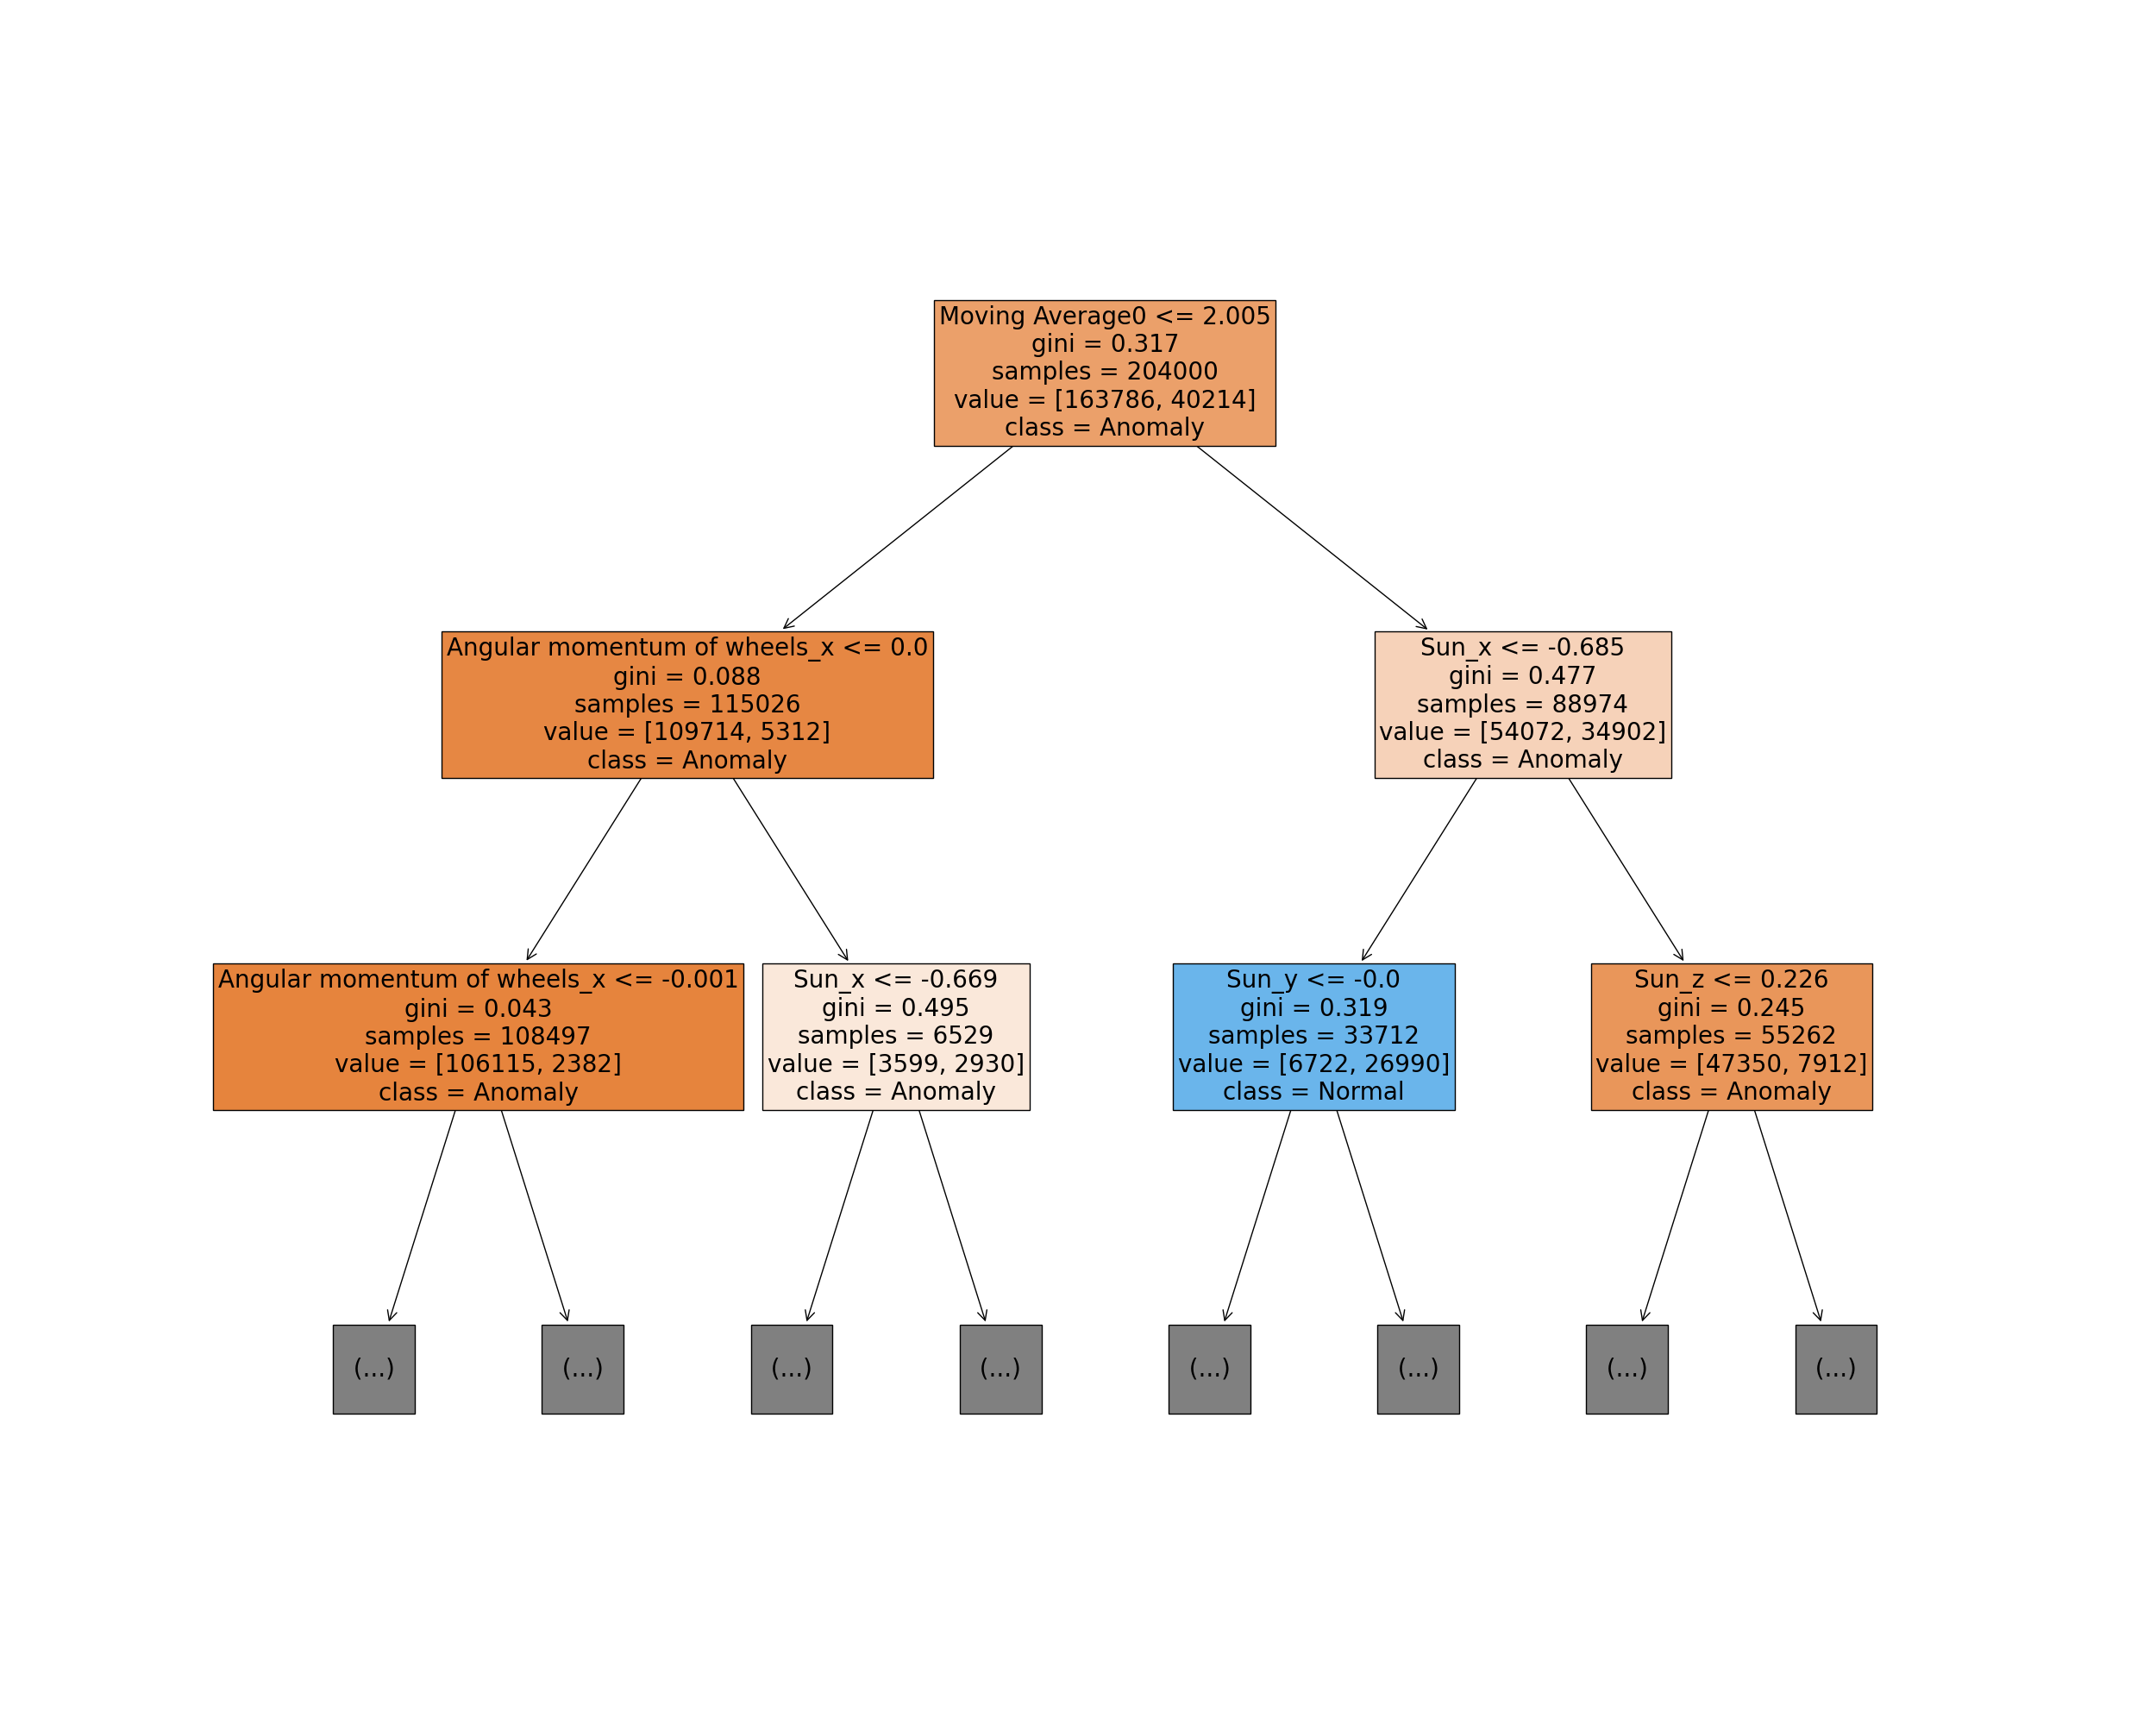
\includegraphics[trim = {3cm 7cm 3cm 7cm},clip, width = 15cm]{/home/ulrich/Documents/Masters thesis/Satellite/Hyperparameters/PhysicsEnabledDMDMethod/DecisionTreeBinaryClass.png}
	\caption{fig:DecisionTree}
\end{figure*}

It is also possible to discuss random forests if it ends up being used in the results, because it is already implemented.


\subsection{Recovery}
Three different methods of recovery are compared. The methods are name Ignore, Backtrack and Replacement. 

The ignore method uses the detected sensor that has failed and ignores the sensor measurement from the EKF measurement update. This method is based on the assumption that the EKF estimation is correct up until the moment where the sensor failure is detected. This method can also have variations, such as the change of the measurement noise covariance matrix $R_k$. This however will dramatically change $K_k$ and will destabilize the EKF rather than stabilizing it. Both methods results however will be discussed in section~\ref{section:Results}.

The backtrack method uses a buffer of $v_{meas,k}$, $v_{model,k}$ and $\hat{x}_k^+$ and other parameters that are used to update the EKF. If a sensor failure is detected, the sensor is excluded from the EKF and the EKF is updated with the sensor data in the buffer excluding the sensor that has failed. The EKF is therefore \emph{reset} and updated from timestep $t_{k-N}$ to $t_k$, where $N$ is the size of the number of timesteps in the buffer. $N$ however must be optimized based on the computational time used to reset the EKF, but still ensure convergence of the EKF. If the sensor that was detected to have anomalous behaviour changes back to normal again, the EKF will be reset once again and the sensor will only be included in the measurement update of $t_k$ since it was anomalous for timesteps before $t_k$.

The replacement methodology changes $v_{meas,k}$ to $v_{est,k}$ at the timestep when the failure is detected. This method depends on the stability and accuracy of the EKF when the failure is detected and highly depends on the accuracy of the detection method. Although this seems to bypass the entire purpose of a measurement update, and might change the change the EKF's dependency to be more on the sensor than the model, even though the sensor measurement might not be accurate. The EKF will remain stable due to the other measurements being accurate and will save computation time. The EKF will not require any reset and the same number of measurements updates will still occur during a sensor's anomalous behaviour.
%
%\begin{figure}[h]
%	\centering
%	\begin{minipage}{0.48\textwidth}
%		\centering
%		\includegraphics[width=0.8\textwidth]{figs/roborace.jpg}
%		
%	\end{minipage}
%	\hfill
%	\begin{minipage}{0.48\textwidth}
%		\centering
%		\includegraphics[width=0.8\textwidth]{figs/KukuMobileRobot.jpg}
%	\end{minipage}
%	
%	\caption{An Autonomous Race Car and Mobile Factory Robot}
%	\label{fig:roborace}
%\end{figure}

\section{Testing methodology}
The testing for the FDIR methods is done by implementing a reflection model on a cubesat from the moment of launching the satellite. Therefore the recovery methods are also implemented from the beginning of the satellite orbit. 

\section{Results}
\label{section:Results}
If sun sensor is the last sensor to be updated in the measurement then a singular matrix error occurs.

Three scenarios are implemented, a satellite that never experiences reflection, a satellite that experiences reflection without any recovery method and a satellite with a recovery method. The subsets of detecting the fault and recovering from the fault will be isolated and discussed separately. Therefore the results for recovery based on perfect detection can be shown to show the possibilities of the recovery method.

The simulation is run for 20 orbits, with each orbit running for 5700$s$. If a fault is induced, it is induced after the first two orbits and the specific anomaly then occurs for the following 18 orbits.

\newpage

\subsection{Perfect Designed Satellite Without Reflection}
\begin{figure}[!htb]
	\centering
	\begin{tikzpicture}
		\centering
		\begin{axis}[width = 7cm, ylabel = $\theta$ (deg), xlabel = Time (s), forget plot style={opacity=0.2}, title = Degrees between reference and actual attitude]
			
			\addplot[line width=1pt,color=blue, each nth point=5, draw opacity=0.7,filter discard warning=false, unbounded coords=discard] table [x expr=\coordindex, y=Pointing Metric, col sep=comma]{/home/ulrich/Documents/Masters thesis/Satellite/Data files/pgfPlots/Predictor-None/Isolator-None/Recovery-None/EARTH_SUN/General CubeSat Model/Metric/None.csv};

		\end{axis}
	\end{tikzpicture}
	\caption[Pointing Accuracy]{Pointing Accuracy.}
	\label{fig:Pointing Accuracy None}
\end{figure}

\begin{figure}[!htb]
	\centering
	\begin{tikzpicture}
		\centering
		\begin{axis}[width = 7cm, ylabel = $\theta$ (deg), xlabel = Time (s), forget plot style={opacity=0.2}, title = Degrees between estimated and actual attitude]
			
			\addplot[line width=1pt,color=blue, each nth point=5, draw opacity=0.7,filter discard warning=false, unbounded coords=discard] table [x expr=\coordindex, y=Estimation Metric, col sep=comma]{/home/ulrich/Documents/Masters thesis/Satellite/Data files/pgfPlots/Predictor-None/Isolator-None/Recovery-None/EARTH_SUN/General CubeSat Model/Metric/None.csv};
			
		\end{axis}
	\end{tikzpicture}
	\caption[Estimation Accuracy]{Estimation Accuracy.}
	\label{fig:Estimation Accuracy None}
\end{figure}
\begin{figure}[!htb]
	\centering
	\begin{tikzpicture}
		\centering
		\begin{axis}[width = 7cm, ylabel = $\theta$ (deg), xlabel = Time (s), forget plot style={opacity=0.2}, title = Degrees between reference and actual attitude]
			
			\addplot[line width=1pt,color=blue, each nth point=5, draw opacity=0.7,filter discard warning=false, unbounded coords=discard] table [x expr=\coordindex, y=Pointing Metric, col sep=comma]{/home/ulrich/Documents/Masters thesis/Satellite/Data files/pgfPlots/Predictor-None/Isolator-None/Recovery-None/EARTH_SUN/General CubeSat Model/Metric/Reflection.csv};
			
		\end{axis}
	\end{tikzpicture}
	\caption[Pointing Accuracy]{Pointing Accuracy.}
	\label{fig:Pointing Accuracy with Reflection and no recovery}
\end{figure}

\begin{figure}[!htb]
	\centering
	\begin{tikzpicture}
		\centering
		\begin{axis}[width = 7cm, ylabel = $\theta$ (deg), xlabel = Time (s), forget plot style={opacity=0.2}, title = Degrees between estimated and actual attitude]
			
			\addplot[line width=1pt,color=blue, each nth point=5, draw opacity=0.7,filter discard warning=false, unbounded coords=discard] table [x expr=\coordindex, y=Estimation Metric, col sep=comma]{/home/ulrich/Documents/Masters thesis/Satellite/Data files/pgfPlots/Predictor-None/Isolator-None/Recovery-None/EARTH_SUN/General CubeSat Model/Metric/Reflection.csv};
			
		\end{axis}
	\end{tikzpicture}
	\caption[Estimation Accuracy]{Estimation Accuracy.}
	\label{fig:Estimation Accuracy with Reflection and no recovery}
\end{figure}
\begin{figure}[!htb]
	\centering
	\begin{tikzpicture}
		\centering
		\begin{axis}[width = 7cm, ylabel = $\theta$ (deg), xlabel = Time (s), forget plot style={opacity=0.2}, title = Degrees between reference and actual attitude]
			
			\addplot[line width=1pt,color=blue, each nth point=5, draw opacity=0.7,filter discard warning=false, unbounded coords=discard] table [x expr=\coordindex, y=Pointing Metric, col sep=comma]{/home/ulrich/Documents/Masters thesis/Satellite/Data files/pgfPlots/Predictor-PERFECT/Isolator-PERFECT/Recovery-EKF/EARTH_SUN/General CubeSat Model/Metric/Reflection.csv};
			
		\end{axis}
	\end{tikzpicture}
	\caption[Pointing Accuracy]{Pointing Accuracy.}
	\label{fig:Pointing Accuracy with PERFECT recovery}
\end{figure}

\begin{figure}[!htb]
	\centering
	\begin{tikzpicture}
		\centering
		\begin{axis}[width = 7cm, ylabel = $\theta$ (deg), xlabel = Time (s), forget plot style={opacity=0.2}, title = Degrees between estimated and actual attitude]
			
			\addplot[line width=1pt,color=blue, each nth point=5, draw opacity=0.7,filter discard warning=false, unbounded coords=discard] table [x expr=\coordindex, y=Estimation Metric, col sep=comma]{/home/ulrich/Documents/Masters thesis/Satellite/Data files/pgfPlots/Predictor-PERFECT/Isolator-PERFECT/Recovery-EKF/EARTH_SUN/General CubeSat Model/Metric/Reflection.csv};
			
		\end{axis}
	\end{tikzpicture}
	\caption[Pointing Accuracy]{Pointing Accuracy.}
	\label{fig:Estimation Accuracy with PERFECT recovery}
\end{figure}
\begin{figure}[!htb]
	\centering
	\begin{tikzpicture}
		\centering
		\begin{axis}[width = 7cm, ylabel = $\theta$ (deg), xlabel = Time (s), forget plot style={opacity=0.2}, title = Degrees between reference and actual attitude]
			
			\addplot[line width=1pt,color=blue, each nth point=5, draw opacity=0.7,filter discard warning=false, unbounded coords=discard] table [x expr=\coordindex, y=Pointing Metric, col sep=comma]{/home/ulrich/Documents/Masters thesis/Satellite/Data files/pgfPlots/Predictor-DecisionTrees/Isolator-DecisionTrees/Recovery-EKF/EARTH_SUN/General CubeSat Model/Metric/Reflection.csv};
			
		\end{axis}
	\end{tikzpicture}
	\caption[Pointing Accuracy]{Pointing Accuracy.}
	\label{fig:Pointing Accuracy Proposed Method}
\end{figure}

\begin{figure}[!htb]
	\centering
	\begin{tikzpicture}
		\centering
		\begin{axis}[width = 7cm, ylabel = $\theta$ (deg), xlabel = Time (s), forget plot style={opacity=0.2}, title = Degrees between estimated and actual attitude]
			
			\addplot[line width=1pt,color=blue, each nth point=5, draw opacity=0.7,filter discard warning=false, unbounded coords=discard] table [x expr=\coordindex, y=Estimation Metric, col sep=comma]{/home/ulrich/Documents/Masters thesis/Satellite/Data files/pgfPlots/Predictor-DecisionTrees/Isolator-DecisionTrees/Recovery-EKF/EARTH_SUN/General CubeSat Model/Metric/Reflection.csv};
			
		\end{axis}
	\end{tikzpicture}
	\caption[Pointing Accuracy]{Pointing Accuracy.}
	\label{fig:Estimation Accuracy Proposed Method}
\end{figure}

\begin{table}[]
	\begin{tabular}{|l|l|l|ll}
		\cline{1-3}
		\multicolumn{1}{|c|}{\textbf{Orbits}} & \textbf{1}         & \textbf{1}         &  &  \\ \cline{1-3}
		\multicolumn{1}{|c|}{Metric}          & Mean               & Std                &  &  \\ \cline{1-3}
		DecisionTrees                         & 18.292514745477845 & 28.632580144211847 &  &  \\ \cline{1-3}
		Perfect                               & 16.472394692952275 & 25.782235910658237 &  &  \\ \cline{1-3}
		None                                  & 16.472394692952275 & 25.782235910658237 &  &  \\ \cline{1-3}
	\end{tabular}
\end{table}

%\csvautotabular{/home/ulrich/Documents/Masters thesis/Satellite/Data files/Summary/Reflection.csv}

Insert a table to compare random orbit parameters. The mean, standard deviation of each orbit 0-20 for each of the different strategies of reflection.

\section{CONCLUSIONS}
Results from kalman filter and attitude determination as well as control compared for EKF with and without FDIR.

\addtolength{\textheight}{-12cm}   % This command serves to balance the column lengths
                                  % on the last page of the document manually. It shortens
                                  % the textheight of the last page by a suitable amount.
                                  % This command does not take effect until the next page
                                  % so it should come on the page before the last. Make
                                  % sure that you do not shorten the textheight too much.

%%%%%%%%%%%%%%%%%%%%%%%%%%%%%%%%%%%%%%%%%%%%%%%%%%%%%%%%%%%%%%%%%%%%%%%%%%%%%%%%



%%%%%%%%%%%%%%%%%%%%%%%%%%%%%%%%%%%%%%%%%%%%%%%%%%%%%%%%%%%%%%%%%%%%%%%%%%%%%%%%



%%%%%%%%%%%%%%%%%%%%%%%%%%%%%%%%%%%%%%%%%%%%%%%%%%%%%%%%%%%%%%%%%%%%%%%%%%%%%%%%
\section*{APPENDIX}
Table of anomalies

\section*{ACKNOWLEDGMENT}




%%%%%%%%%%%%%%%%%%%%%%%%%%%%%%%%%%%%%%%%%%%%%%%%%%%%%%%%%%%%%%%%%%%%%%%%%%%%%%%%

References are important to the reader; therefore, each citation must be complete and correct. If at all possible, references should be commonly available publications.

% \begin{thebibliography}{99}

% \bibitem{c1} G. O. Young, ÒSynthetic structure of industrial plastics (Book style with paper title and editor),Ó 	in Plastics, 2nd ed. vol. 3, J. Peters, Ed.  New York:  % McGraw-Hill, 1964, pp. 15Ð64.
% \bibitem{c2} W.-K. Chen, Linear Networks and Systems (Book style).	Belmont, CA: Wadsworth, 1993, pp. 123Ð135.






% \end{thebibliography}


\end{document}
